\documentclass[10pt]{beamer}
\usepackage{uglixbeamer}
\title{CH04 - Bases de données}
\subtitle{Partie 3}
\author{T$^{\text{ale}}$ NSI}
\usepackage[normalem]{ulem}
\setminted{bgcolor= codebackground,fontsize=\footnotesize}
\setmintedinline{bgcolor= beamerWhite,fontsize=\normalsize}

\begin{document}
	\maketitle
    \section{Niveau physique\\ Langage SQL}
\begin{frame}{Le SGBD}
Il garantit entre autres\pause
\begin{itemize}
	\item	\alert{l'indépendance physique} de la BDD : l'utilisateur n'a pas à se soucier des aspects matériels;\pause
	\item	\alert{l'indépendance logique} : les programmes qui utilisent la BDD sont indépendants de sa structure logique;\pause
    \item 	\alert{l'accès aux données} : il se fait grâce à un \alert{langage de manipulation des données} (LMD) optimisé pour la rapidité et l'accès simultané multiple en lecture/écriture;\pause
    \item 	\alert{la centralisation des données pour administration};\pause
    \item 	\alert{la non-redondance des données};\pause
    \item 	\alert{la sécurité des données} vis-à-vis du piratage mais aussi des pannes physiques.
\end{itemize}
\end{frame}

\begin{frame}{Principaux SGBD en 2020}
	
\includegraphics[width=3cm]{img/mysql}\ \ \ \ \ \ 
\includegraphics[width=3cm]{img/postgresql}\ \ \ \ \ \ 
\includegraphics[width=3cm]{img/microsoftsqlserver}\\

	
\includegraphics[width=3cm]{img/sqlite}\ \ \ \ \ \ 
\includegraphics[width=3cm]{img/oracle}\ \ \ \ \ \ 
\includegraphics[width=3cm]{img/mongodb}

\end{frame}
\begin{frame}{Le SQL}
\begin{itemize}
    \item	\textit{Structured Query Langage} (langage de requêtes structuré).\pause
	\item	Créé en 1974, normalisé en 1986, dernière version parue en 2011.\pause
    \item 	Utilisé par la plupart des SGBD avec de petites différences.
\end{itemize}

\end{frame}

\begin{frame}[fragile]{Exemple de requête}

\footnotesize

\begin{minted}{sql}
SELECT DISTINCT nom, prenom
FROM Auteur
         JOIN Ecrire ON Ecrire.id_auteur = Auteur.id_auteur
         JOIN Livre ON Livre.num_isbn = Ecrire.num_isbn
WHERE Livre.titre LIKE '%s%';
\end{minted}

\normalsize\pause
Voici comment obtenir la liste des noms et prénoms des auteurs ayant écrit un livre dont le titre comporte la lettre \og s\fg{}. Nous expliquerons comment produire de telles requêtes plus tard.
\end{frame}
\begin{frame}{Vocabulaire}
	En SQL, les relations s'appellent des \alert{tables}.\\\pause

	Les éléments des tables s'appellent des \alert{tuples}.
\end{frame}
\begin{frame}{Bilan des termes utilisés}
\begin{center}
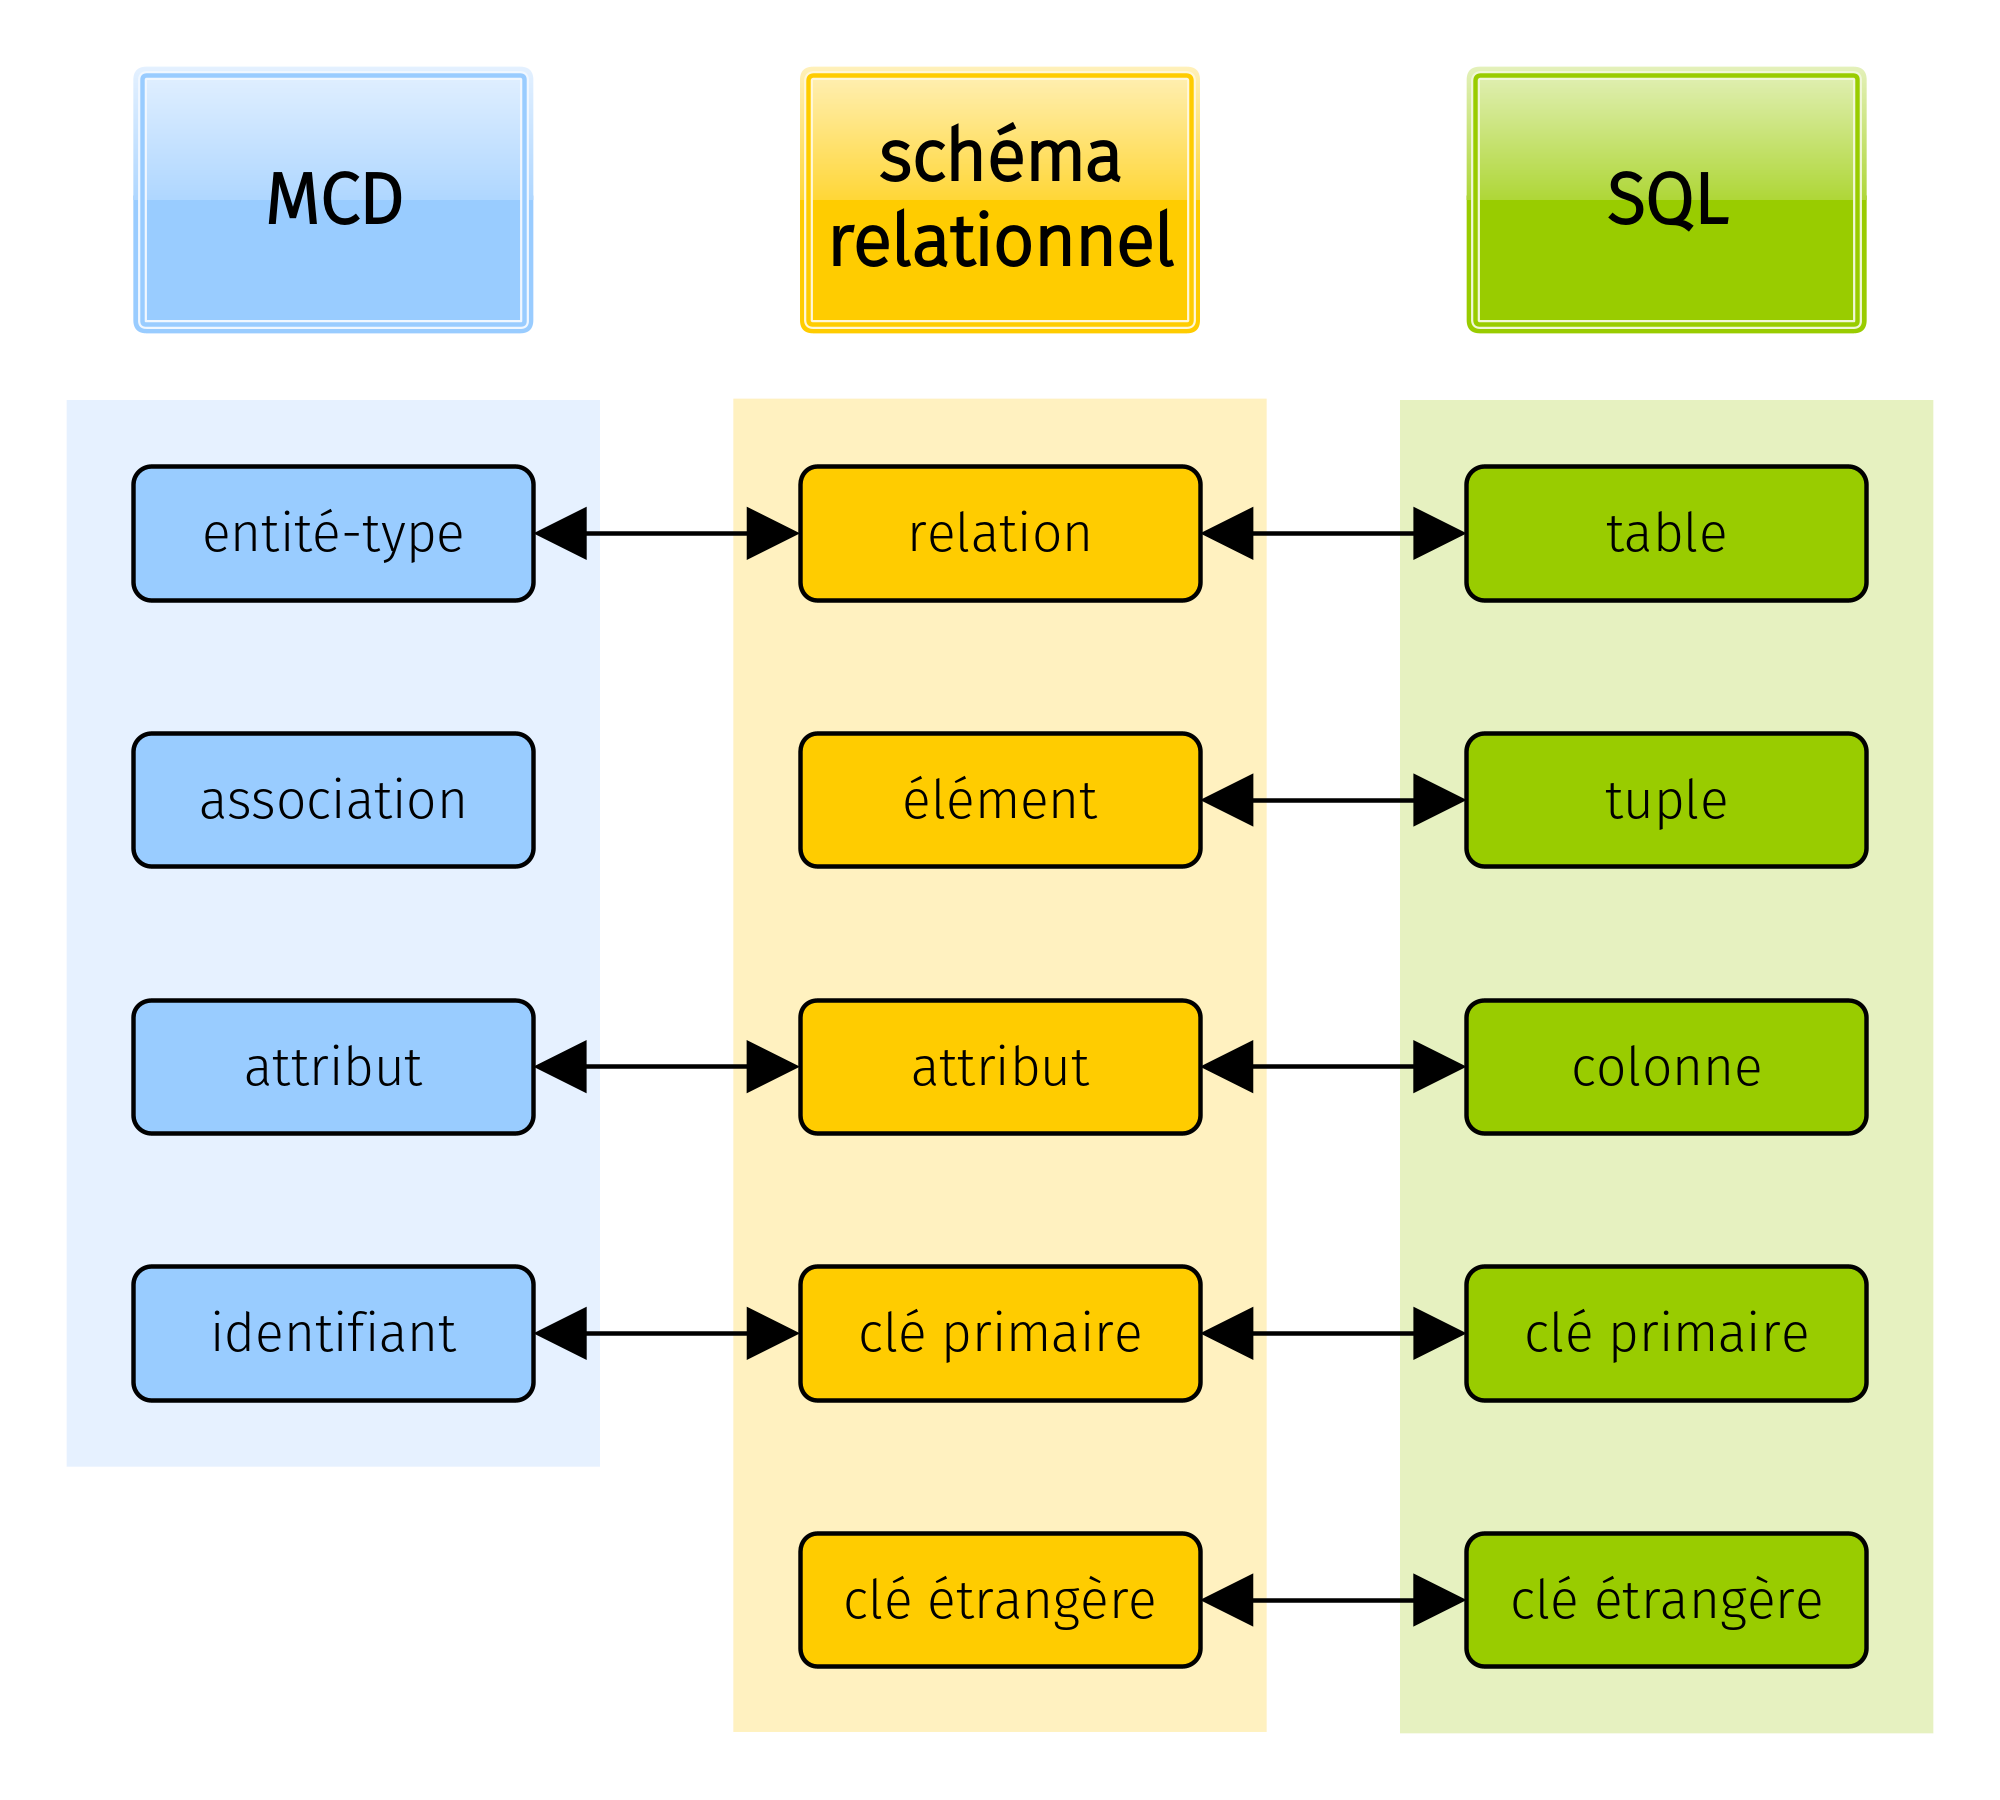
\includegraphics[width=9cm]{img/classification}
\end{center}
\end{frame}
\begin{frame}{Conventions}
	On écrira les mots-clés SQL en majuscules.\\\pause

	On ne met pas d'accents ou d'espaces dans les noms des tables ou des attributs.\\\pause

    Les espaces et tabulations n'ont qu'un rôle esthétique.\\\pause

	Les requêtes peuvent prendre plusieurs lignes mais doivent se terminer par un point-virgule.\\\pause

	On utilisera SQLite car on peut s'en servir avec DB Browser sans installation compliquée.
\end{frame}
\section{Création de la BDD}
\begin{frame}[fragile]{Créer une BDD}

\begin{minted}{sql}
CREATE DATABASE Bibliotheque;
USE Bibliotheque;
\end{minted}
\pause
On n'utilisera pas cette commande : dans DB	Browser on peut créer un nouveau fichier de BDD sans passer par SQLite.
\end{frame}

\begin{frame}[fragile]{Supprimer une BDD}

	\begin{minted}{sql}
DROP DATABASE Bibliotheque;
	\end{minted}
\pause
	On n'utilisera pas cette commande non plus.
\end{frame}

\begin{frame}[fragile]{Créer une table}
Voici comment créer la table \textbf{Pays} :

\begin{minted}{sql}
DROP TABLE IF EXISTS Pays; -- recréer la table de zéro
CREATE TABLE Pays
(
    nom_pays   TEXT,
    population INTEGER,
    superficie INTEGER,
    PRIMARY KEY (nom_pays), -- clé primaire
    CHECK (population > 0), -- contraintes utilisateur
    CHECK (superficie > 0)
);
\end{minted}

\end{frame}

\begin{frame}[fragile]{Table \textbf{Livre}}


\begin{minted}{sql}
DROP TABLE IF EXISTS Livre;
CREATE TABLE Livre
(
    num_isbn INTEGER,
    titre    TEXT,
    annee    TEXT,
    PRIMARY KEY (num_isbn),
    CHECK (date(annee) BETWEEN '1900' AND '2100')
);
\end{minted}
\pause
\mintinline{sql}{date(annee) BETWEEN '1900' AND '2100'} est l'équivalent SQL de\mintinline{python}{'1900' <= date(annee) <= '2100'} en Python.\pause
\begin{alertblock}{Attention}
SQLite ne connaît pas le type \mintinline{sql}{DATE}, il faut créer des attributs de type \mintinline{sql}{TEXT} et utiliser la fonction \mintinline{sql}{date}.
\end{alertblock}
\end{frame}
\begin{frame}[fragile]{Table \textbf{Livre}}
\begin{minted}{sql}
DROP TABLE IF EXISTS Auteur;
CREATE TABLE Auteur
(
    id_auteur      INTEGER,
    nom_pays       TEXT,
    nom            TEXT,
    prenom         TEXT,
    date_naissance TEXT,
    PRIMARY KEY (id_auteur),
    UNIQUE (nom, prenom), -- contrainte d'unicité
    FOREIGN KEY (nom_pays) REFERENCES Pays (nom_pays)
    /*nom_pays est une clé étrangère*/
        ON DELETE CASCADE
        /*si on supprime des tuples dans Pays, automatiquement
        (en cascade) on supprimera les tuples qui y font
        réference dans Auteur*/
        ON UPDATE CASCADE
        /*si on met à jour les attributs nom_pays dans Pays,
        alors le SGBD les mettra à jour aussi dans Auteur*/
);\end{minted}
\end{frame}
\begin{frame}{Ordre des créations des tables}
	On ne peut pas créer \textbf{Auteur} avant d'avoir crée \textbf{Pays} car \textbf{Auteur} possède une clé étrangère liée à \textbf{Pays}.
\end{frame}

\begin{frame}[fragile]{Table \textbf{Ecrire}}
\begin{minted}{sql}
DROP TABLE IF EXISTS Ecrire;
CREATE TABLE Ecrire
(
    id_auteur    INTEGER,
    num_isbn     INTEGER,
    nb_chapitres INTEGER,
    PRIMARY KEY (id_auteur, num_isbn),
    FOREIGN KEY (id_auteur) REFERENCES Auteur (id_auteur)
        ON DELETE CASCADE
        ON UPDATE CASCADE,
    FOREIGN KEY (num_isbn) REFERENCES Livre (num_isbn)
            ON DELETE CASCADE
            ON UPDATE CASCADE
);
\end{minted}
\end{frame}
\section{Variantes syntaxiques et autres}
\begin{frame}[fragile]{\'Ecriture plus compacte}
On peut signifier qu'un attribut est une clé étrangère dans sa définition même :\pause
\begin{minted}{sql}
DROP TABLE IF EXISTS Ecrire;
CREATE TABLE Ecrire
(
    id_auteur    INTEGER REFERENCES Auteur (id_auteur)
        ON DELETE CASCADE
        ON UPDATE CASCADE,
    num_isbn     INTEGER REFERENCES Livre (num_isbn)
        ON DELETE CASCADE
        ON UPDATE CASCADE,
    nb_chapitres INTEGER,
    PRIMARY KEY (id_auteur, num_isbn)
);
\end{minted}
\end{frame}

\begin{frame}[fragile]{\'Ecriture plus compacte (bis)}
On peut signifier qu'un attribut est une clé primaire dans sa définition même :\pause
\begin{minted}{sql}
DROP TABLE IF EXISTS Livre;
CREATE TABLE Livre
(
    num_isbn INTEGER PRIMARY KEY,
    titre    TEXT,
    annee    TEXT,
    CHECK (date(annee) BETWEEN '1900' AND '2100')
);
\end{minted}
\end{frame}


\section{Insertion des données dans la BDD}


\begin{frame}[fragile]{Données de \textbf{Pays}}
\begin{minted}{sql}
INSERT INTO Pays
VALUES ('France', 672051, 67064000),
       ('Italie', 301336, 66436000),
       ('Royaume-Uni', 242900, 60317000);
\end{minted}
Les attributs des tuples sont dans le même ordre que lors de la création.
\end{frame}

\begin{frame}{\textit{Et c\ae tera}}
	De même que lors de la création, on ne peut pas insérer de tuples dans \textbf{Auteur} avant d'avoir peuplé \textbf{Pays} : en effet dans un tuple de \textbf{Auteur} tel que \\

    \mintinline{sql}{(1, 'France', 'Hugo', 'Victor', '1802-02-26')}\\

    Les contraintes de référence font qu'un tuple \og France\fg{} doit d'abord exister dans \textbf{Pays}.
\end{frame}
\end{document}